\documentclass[11pt,a4paper]{article}
\usepackage[utf8]{inputenc}
\usepackage[vietnamese]{babel}
\usepackage{amsmath,amssymb}
\usepackage[version=4]{mhchem}
\usepackage{geometry}
\geometry{top=1.5cm,bottom=1.2cm,left=1.4cm,right=1.4cm,headheight=28pt,headsep=12pt,footskip=18pt}
\usepackage{graphicx}
\usepackage{xcolor}
\usepackage{tabularx}
\usepackage{array}
\usepackage{tikz}
\usepackage{fancyhdr}
\usepackage{enumitem}
\usepackage{multido}
\usepackage{tcolorbox}

\definecolor{hfRed}{HTML}{D32F2F}
\definecolor{hfGreen}{HTML}{8BC390}
\definecolor{mainGreen}{HTML}{2E7D32}
\definecolor{solBlue}{HTML}{1565C0}
\definecolor{tableGreen}{HTML}{E8F5E9}

\usepackage{ex_test}

\pagestyle{fancy}
\fancyhf{}
\renewcommand{\headrulewidth}{0.75pt}
\renewcommand{\headrule}{\hbox to\headwidth{\color{hfGreen}\leaders\hrule height \headrulewidth\hfill}}
\renewcommand{\footrulewidth}{0.75pt}
\renewcommand{\footrule}{\hbox to\headwidth{\color{hfGreen}\leaders\hrule height \footrulewidth\hfill}}

\fancyhead[L]{\small\itshape\color{hfRed}Tài liệu lưu hành nội bộ}
\fancyhead[R]{\small\color{hfRed}Thầy \textbf{TRẦN VĂN THẠNH} - 0777.470.803}

\fancyfoot[L]{\footnotesize\itshape\color{hfRed}CS1: 6/15 Nguyễn Hoàng, P. Kim Long, TP Huế \quad|\quad CS2: 24 Đặng Thái Thân, TP Huế}
\fancyfoot[R]{\small\textbf{\color{hfRed}Trang \thepage}}

\setlength{\parindent}{0pt}
\setlength{\parskip}{2pt}

\begin{document}

\begin{minipage}[t]{0.48\textwidth}
\textbf{SỞ GD\&ĐT THỪA THIÊN HUẾ}\\
\textbf{TRƯỜNG THPT HAI BÀ TRƯNG}\\
\textit{ĐỀ CHÍNH THỨC}\\
\textit{(Đề thi có 03 trang)}
\end{minipage}
\hfill
\begin{minipage}[t]{0.48\textwidth}
\raggedleft
\textbf{\color{hfRed}ĐỀ KIỂM TRA GIỮA KÌ I - NĂM HỌC 2024 - 2025}\\
\textbf{MÔN: HOÁ HỌC -- LỚP 10}\\
\textit{Thời gian làm bài: 45 phút (không kể thời gian phát đề)}\\
\textbf{MÃ ĐỀ: GỐC}
\end{minipage}

\vspace{4pt}
\noindent
\textit{Họ, tên thí sinh:} \dotfill \textit{Lớp:} \dotfill \textit{Số báo danh:} \dotfill

\vspace{3pt}
\noindent
\textit{\footnotesize Cho NTK: $\ce{Na=23; K=39; Mg=24; Ca=40; Ba=137; Al=27; Cl=35,5; H=1; C=12; O=16; N=14}$.\\
(Học sinh không sử dụng bảng hệ thống tuần hoàn các nguyên tố hóa học)}

\vspace{3pt}
\hrule color{hfGreen} height 0.5pt

\vspace{4pt}
\noindent
{\color{mainGreen}\textbf{\Large A. PHẦN TRẮC NGHIỆM: (7,0 điểm)}}

\vspace{3pt}
\noindent
{\color{mainGreen}\textbf{\large PHẦN I (3,0 điểm). TRẮC NGHIỆM NHIỀU LỰA CHỌN}}\\
\textit{\small Thí sinh trả lời từ câu 1 đến câu 12. Mỗi câu hỏi thí sinh chỉ chọn một phương án.}
\vspace{2pt}

\begin{ex}
Nội dung nào dưới đây không phải là đối tượng nghiên cứu của hóa học ?
\choice
{Thành phần, cấu trúc của chất.}
{Tính chất và sự biến đổi của chất.}
{Ứng dụng của chất.}
{\True Sự lớn lên và sinh sản của tế bào.}
\end{ex}
\begin{ex}
Nguyên tử chứa những hạt mang điện là
\choice
{proton và neutron.}
{\True proton và electron.}
{electron và neutron.}
{electron và hạt alpha.}
\end{ex}
\begin{ex}
Chọn đáp án sai
\choice
{Proton, $m \approx 1\text{ amu}, q = +1$.}
{Electron, $m \approx 0,00055\text{ amu}, q = -1$.}
{Neutron, $m \approx 1\text{ amu}, q = 0$.}
{\True Electron, $m \approx 1\text{ amu}, q = -1$.}
\end{ex}
\begin{ex}
Thông tin nào sau đây không đúng về $^{28}_{14}\ce{N}$ (hoặc $^{28}_{14}\ce{Si}$)?
\choice
{Số khối là 28.}
{Tổng số proton và neutron là 28.}
{\True Số neuton là 28.}
{Số đơn vị điện tích hạt nhân là 14.}
\end{ex}
\begin{ex}
Nguyên tử của nguyên tố X có 56 electron trong lớp vỏ, 82 neutron trong hạt nhân. Kí hiệu của nguyên tử nguyên tố X là
\choice
{$^{56}_{82}\ce{A}$.}
{$^{82}_{56}\ce{A}$.}
{$^{56}_{138}\ce{A}$.}
{\True $^{138}_{56}\ce{A}$.}
\end{ex}
\begin{ex}
Phát biểu nào sau đây không đúng
\choice
{Orbital nguyên tử được kí hiệu là AO (Atomic Orbital).}
{Theo mô hình hiện đại, trong nguyên tử, electron chuyển động rất nhanh, không theo quỹ đạo xác định.}
{\True Có 3 loại orbital nguyên tử: orbital s, orbital p và orbital d.}
{Các orbital s có dạng hình cầu và orbital p có dạng hình số 8 nổi.}
\end{ex}
\begin{ex}
Lớp N có số phân lớp electron bằng
\choice
{1.}
{2.}
{3.}
{\True 4.}
\end{ex}
\begin{ex}
Nguyên tử nguyên tố M có số hiệu nguyên tử bằng 20. Cấu hình electron của ion $\ce{M^{2+}}$ là
\choice
{$\ce{1s^2 2s^2 2p^6 3s^2 3p^6 4s^2}$.}
{\True $\ce{1s^2 2s^2 2p^6 3s^2 3p^6}$.}
{$\ce{1s^2 2s^2 2p^6 3s^2 3p^6 3d^2 4s^2}$.}
{$\ce{1s^2 2s^2 2p^8 3s^2 3p^6}$.}
\end{ex}
\begin{ex}
Chu kì là dãy các nguyên tố được xếp theo chiều điện tích hạt nhân tăng dần, nguyên tử của chúng có cùng
\choice
{số electron ở lớp ngoài cùng.}
{\True số lớp electron.}
{số electron hóa trị.}
{số electron.}
\end{ex}
\begin{ex}
Nguyên tố Y thuộc chu kì 4, nhóm IA của bảng tuần hoàn. Phát biểu nào sau đây về Y là đúng ?
\choice
{Y có độ âm điện lớn nhất và bán kính nguyên tử nhỏ nhất trong chu kì 4.}
{Y có độ âm điện lớn nhất và bán kính nguyên tử lớn nhất trong chu kì 4.}
{\True Y có độ âm điện nhỏ nhất và bán kính nguyên tử lớn nhất trong chu kì 4.}
{Y có độ âm điện nhỏ nhất và bán kính nguyên tử nhỏ nhất trong chu kì 4.}
\end{ex}
\begin{ex}
Trong một chu kì, bán kính nguyên tử
\choice
{xấp xỉ bằng nhau.}
{biến đổi ngẫu nhiên.}
{tăng theo chiều tăng dần của điện tích hạt nhân.}
{\True giảm theo chiều tăng dần của điện tích hạt nhân.}
\end{ex}
\begin{ex}
Cho các nguyên tố sau: $\ce{Li}\ (Z=3),\ \ce{O}\ (Z=8),\ \ce{F}\ (Z=9),\ \ce{Na}\ (Z=11)$. Dãy gồm các nguyên tố được sắp xếp theo chiều tăng dần bán kính nguyên tử từ trái sang phải là
\choice
{F, Li, O, Na.}
{Li, Na, O, F.}
{F, Na, O, Li.}
{\True F, O, Li, Na.}
\end{ex}
\vspace{4pt}
\noindent
{\color{mainGreen}\textbf{\large PHẦN II (2,0 điểm). CÂU TRẮC NGHIỆM ĐÚNG / SAI}}\\
\textit{\small Thí sinh trả lời từ câu 1 đến câu 2. Trong mỗi ý a), b), c), d) ở mỗi câu, thí sinh chọn đúng (Đ) hoặc sai (S).}
\vspace{2pt}

\begin{ex}
Các phát biểu sau đây là đúng hay sai?
\choiceTF
{Nguyên tử của nguyên tố hydrogen luôn có 2 proton}
{\True Nguyên tử của nguyên tố hydrogen có thể không có neutron}
{Nếu đường kính của nguyên tử khoảng $10^2\text{ pm}$ thì đường kính của hạt nhân khoảng $10^{-4}\text{ pm}$}
{Nguyên tố hóa học là tập hợp các nguyên tử có cùng số neutron trong hạt nhân}
\end{ex}
\begin{ex}
Cho sơ đồ của một nguyên tử X được biểu diễn như hình bên:
\begin{center}
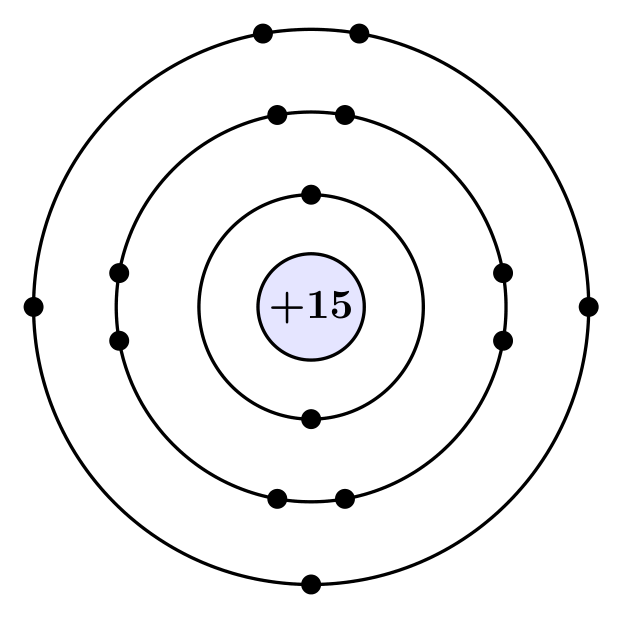
\includegraphics[width=4.5cm]{images_hoa10/so_do_nguyen_tu_p_15.png}
\end{center}
\choiceTF
{Các electron trong nguyên tử X chỉ được phân bố trên 2 lớp K và lớp L}
{\True Ở trạng thái cơ bản, nguyên tử X có 3 electron độc thân}
{Nguyên tử nguyên tố X có tổng số hạt cơ bản là 50 hạt. Số hạt mang điện nhiều hơn số hạt không mang điện là 10 hạt. Số hạt neutron của X là 35}
{\True X thuộc ô 15, chu kỳ 3, nhóm VA}
\end{ex}
\vspace{4pt}
\noindent
{\color{mainGreen}\textbf{\large PHẦN III (2,0 điểm). CÂU TRẮC NGHIỆM TRẢ LỜI NGẮN}}\\
\textit{\small Thí sinh trả lời từ câu 1 đến câu 4.}
\vspace{2pt}

\begin{ex}
Cho dãy nguyên tố sau: Na (1), K (2), Rb (3), Li (4). Hãy sắp xếp theo chiều giảm dần bán kính nguyên tử? (ghi thứ tự các số)

\noindent\textit{Trả lời:} \dotfill
\end{ex}
\begin{ex}
Cho số hiệu nguyên tử của $\ce{Li}\ (Z=3),\ \ce{Na}\ (Z=11),\ \ce{P}\ (Z=15),\ \ce{Ar}\ (Z=18)$. Có bao nhiêu nguyên tố p trong các nguyên tố trên?

\noindent\textit{Trả lời:} \dotfill
\end{ex}
\begin{ex}
Đồng vị phóng xạ cobalt ($^{60}_{27}\ce{Co}$) phát ra tia $\gamma$ có khả năng đâm xuyên mạnh, dùng điều trị các khối u ở sâu trong cơ thể. Cobalt có ba đồng vị: $^{59}_{27}\ce{Co}$ (chiếm 98\%), $^{58}_{27}\ce{Co}$ và $^{60}_{27}\ce{Co}$; nguyên tử khối trung bình là 58,982. Xác định hàm lượng \% của đồng vị phóng xạ $^{60}_{27}\ce{Co}$.

\noindent\textit{Trả lời:} \dotfill
\end{ex}
\begin{ex}
Nguyên tử X có tổng số hạt cơ bản là 49, số hạt không mang điện bằng 53,125\% số hạt mang điện. Số neutron của nguyên tử X là bao nhiêu?

\noindent\textit{Trả lời:} \dotfill
\end{ex}
\vspace{6pt}
\noindent
{\color{mainGreen}\textbf{\Large B. PHẦN TỰ LUẬN: (3,0 điểm)}}
\vspace{2pt}

\noindent
\textbf{Câu 1 (1,0 điểm):} Cho nguyên tố A có số hiệu nguyên tử $Z = 13$.\\
a) Viết cấu hình electron nguyên tử của nguyên tố A. Cho biết A là kim loại, phi kim hay khí hiếm?\\
b) Biểu diễn cấu hình electron của A theo ô orbital. Cho biết số electron độc thân của nguyên tử A?

\vspace{1pt}
\noindent
\multido{\n=1+1}{6}{\dotfill\\[4pt]}

\vspace{4pt}
\noindent
\textbf{Câu 2 (1,0 điểm):} Kim loại M thuộc nhóm IIA của bảng tuần hoàn, là một thành phần dinh dưỡng quan trọng. Sự thiếu hụt rất nhỏ của nó đã ảnh hưởng tới sự hình thành và phát triển của xương, răng. Thừa M có thể dẫn đến sỏi thận. Cho 1,2 gam M tác dụng hết với dung dịch HCl, thu được 0,7437 L khí (đkc).\\
a) Xác định M và viết cấu hình electron của ion $\ce{M^{2+}}$.\\
b) Sắp xếp theo thứ tự tăng dần về bán kính nguyên tử của nguyên tố M với $_{19}\ce{K}$ và $_{12}\ce{Mg}$.

\vspace{1pt}
\noindent
\multido{\n=1+1}{7}{\dotfill\\[4pt]}

\vspace{4pt}
\noindent
\textbf{Câu 3 (1,0 điểm):} Trong tự nhiên nguyên tố X có hai đồng vị là $^{35}_{17}\ce{X}$ và đồng vị thứ hai $^{37}_{17}\ce{X}$. Biết nguyên tử khối trung bình của X là 35,48.\\
a) Xác định vị trí của X trong bảng tuần hoàn (ô, chu kì, nhóm)?\\
b) Tính \% số nguyên tử của đồng vị $^{35}_{17}\ce{X}$.

\vspace{1pt}
\noindent
\multido{\n=1+1}{6}{\dotfill\\[4pt]}

\vspace{6pt}
\begin{center}
\textbf{---------- HẾT ----------}\\
\textit{\small (Thí sinh không được sử dụng tài liệu. Cán bộ coi thi không giải thích gì thêm)}
\end{center}

\end{document}
